\documentclass{article}
\usepackage[a4paper,top=3cm,bottom=3cm,left=3cm,right=3cm]{geometry}
\usepackage{graphicx}
\usepackage{tikz}
\usetikzlibrary{shapes.geometric,arrows.meta,positioning,fit,backgrounds,calc}
\usepackage{amsmath}

\begin{document}
\pagestyle{empty}

\noindent
\resizebox{\linewidth}{!}{%
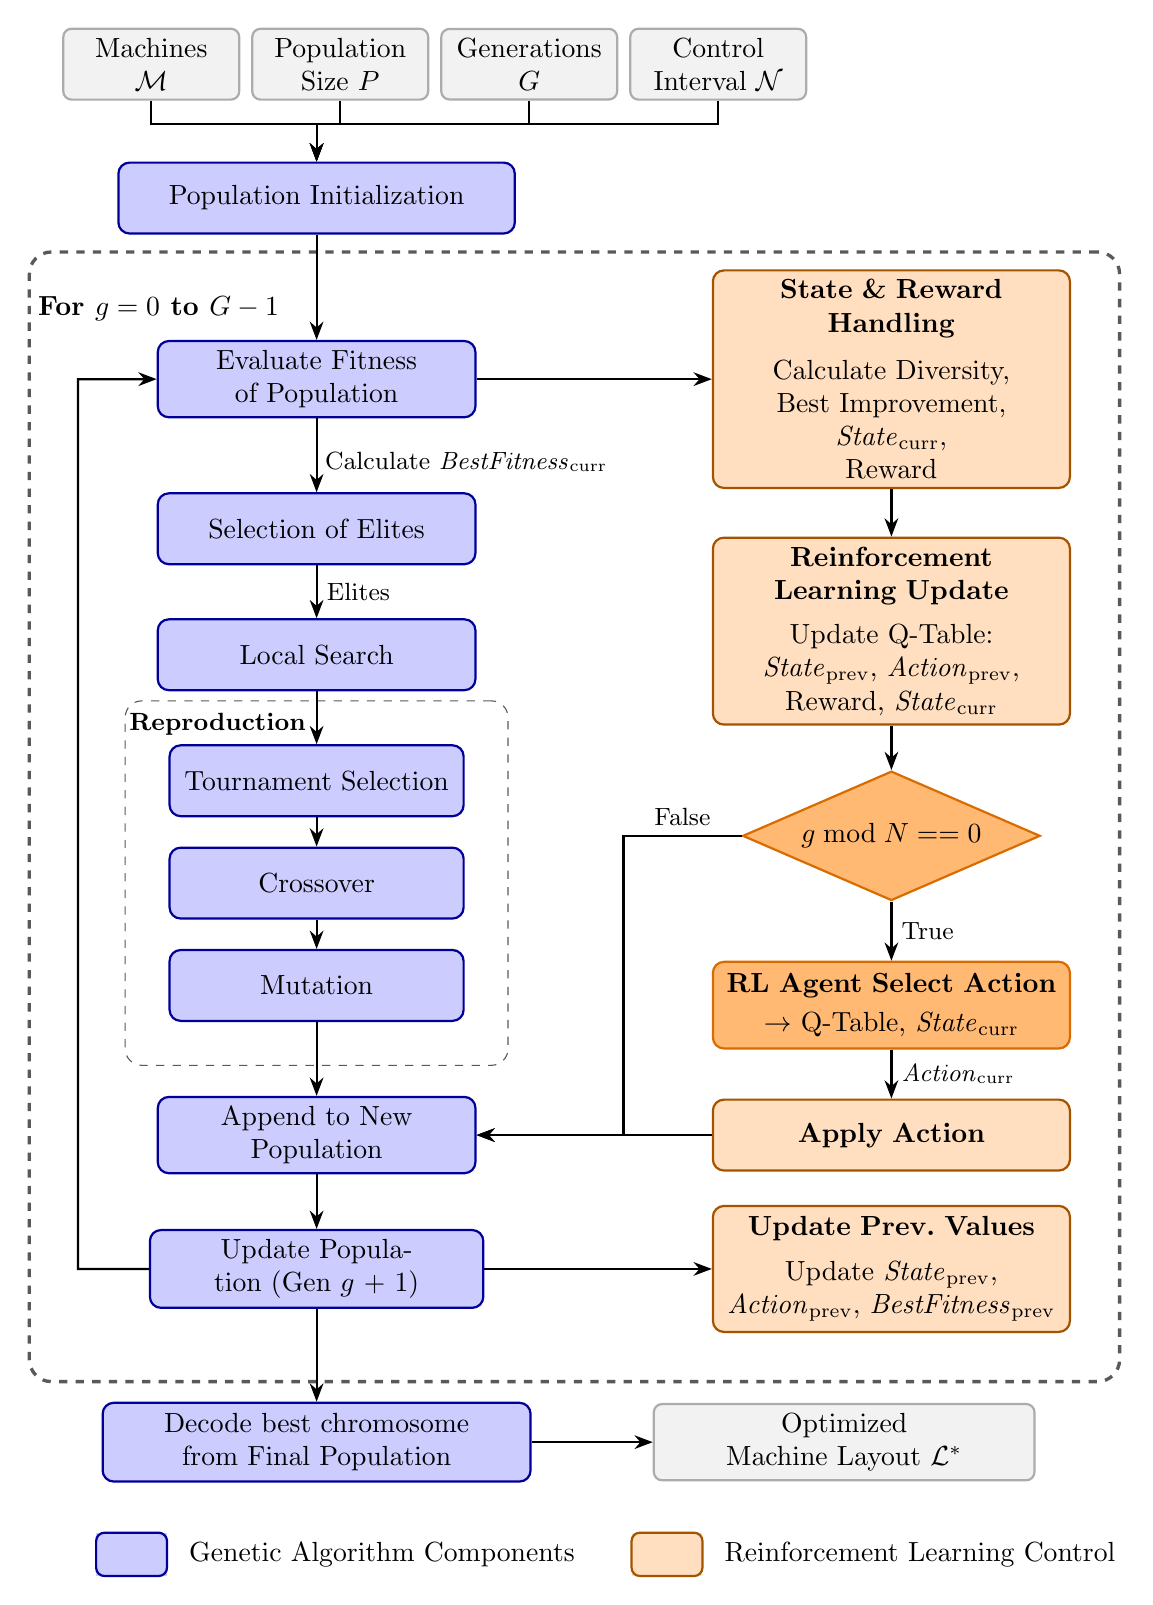
\begin{tikzpicture}[x=1cm, y=1cm, thick, >=Stealth,
  %-------- box styles --------
  gabox/.style={
    rectangle, rounded corners=4pt,
    draw=blue!60!black, fill=blue!20,
    minimum height=0.9cm, align=center
  },
  rlbox/.style={
    rectangle, rounded corners=4pt,
    draw=orange!65!black, fill=orange!25,
    align=center
  },
  rlboxd/.style={
    rectangle, rounded corners=4pt,
    draw=orange!85!black, fill=orange!55,
    minimum height=0.9cm, align=center
  },
  inpbox/.style={
    rectangle, rounded corners=3pt,
    draw=gray!65, fill=gray!10,
    minimum height=0.65cm, align=center
  },
  outbox/.style={
    rectangle, rounded corners=3pt,
    draw=gray!65, fill=gray!10,
    minimum height=0.65cm, align=center
  },
  diam/.style={
    diamond, draw=orange!85!black, fill=orange!55,
    aspect=2.3, minimum width=3.1cm, minimum height=0.9cm, align=center
  },
]

%%=============================================================
%% INPUTS ROW  (y = 22.5)
%%=============================================================
\node[inpbox, text width=2.0cm] (MACH)    at (1.9,  23) {Machines \\ $\mathcal{M}$};
\node[inpbox, text width=2.0cm] (POPSIZE) at (4.3,  23) {Population\\ Size $P$};
\node[inpbox, text width=2.0cm] (GENS)    at (6.7,  23) {Generations $G$};
\node[inpbox, text width=2.0cm] (CTRL)    at (9.1,  23) {Control\\ Interval $\mathcal{N}$};

%%=============================================================
%% POPULATION INITIALIZATION  (y = 20.8)
%%=============================================================
\node[gabox, text width=4.8cm] (POPINIT) at (4.0, 21.3)
  {Population Initialization};

\draw[->] (MACH.south)    -- ++(0,-0.3) -| (POPINIT.north);
\draw[->] (POPSIZE.south) -- ++(0,-0.3) -| (POPINIT.north);
\draw[->] (GENS.south)    -- ++(0,-0.3) -| (POPINIT.north);
\draw[->] (CTRL.south)    -- ++(0,-0.3) -| (POPINIT.north);

%%=============================================================
%% GA COLUMN  (centre x = 4.0)
%%=============================================================

%% Evaluate Fitness  (y = 19.0)
\node[gabox, text width=3.8cm] (EVALFIT) at (4.0, 19.0)
  {Evaluate Fitness\\ of Population};

% POPINIT → EVALFIT
\draw[->] (POPINIT.south) -- ++(0,-0.5) -| (EVALFIT.north);

% "Calculate BestFitness_curr" annotation (between EVALFIT and SELELITE)
\node[font=\small, align=center] at (5.9, 17.95)
  {Calculate $\mathit{BestFitness}_\mathrm{curr}$};

%% Selection of Elites  (y = 17.1)
\node[gabox, text width=3.8cm] (SELELITE) at (4.0, 17.1)
  {Selection of Elites};
\draw[->] (EVALFIT.south) -- (SELELITE.north);

%% Local Search  (y = 15.5)
\node[gabox, text width=3.8cm] (LOCSEARCH) at (4.0, 15.5)
  {Local Search};
\draw[->] (SELELITE.south) -- node[right, font=\small] {Elites} (LOCSEARCH.north);

%%--- Reproduction box: Tournament / Crossover / Mutation ---

\node[gabox, text width=3.5cm] (TOURNAMENT) at (4.0, 13.9)
  {Tournament Selection};
\node[gabox, text width=3.5cm] (CROSSOVER)  at (4.0, 12.6)
  {Crossover};
\node[gabox, text width=3.5cm] (MUTATION)   at (4.0, 11.3)
  {Mutation};

\draw[->] (LOCSEARCH.south) -- (TOURNAMENT.north);
\draw[->] (TOURNAMENT.south) -- (CROSSOVER.north);
\draw[->] (CROSSOVER.south)  -- (MUTATION.north);

% Loop arrow inside reproduction box: MUTATION right side → up → TOURNAMENT right side
% \draw[->] (MUTATION.east) -- ++(0.5, 0) |- (TOURNAMENT.east);

%% Dashed REPRODUCTION box
\begin{scope}[on background layer]
  \node[draw=black!65, dashed, rounded corners=6pt, inner sep=0.55cm,
        fit=(TOURNAMENT)(CROSSOVER)(MUTATION)] (REPBOX) {};
\end{scope}
\node[font=\small\bfseries, anchor=north west, xshift=-2pt, yshift=-1pt]
  at (REPBOX.north west)
  {\textbf{Reproduction}};

%% Assemble NewPop  (y = 9.4)
\node[gabox, text width=3.8cm] (ASSEMBLENP) at (4.0, 9.4)
  {Append to New Population};
\draw[->] (MUTATION.south) -- ++(0,-0.65) -- (ASSEMBLENP.north);

%% Update Population  (y = 7.7)
\node[gabox, text width=4.0cm] (UPDATEPOP) at (4.0, 7.7)
  {Update Population (Gen $g+1$)};
\draw[->] (ASSEMBLENP.south) -- (UPDATEPOP.north);

%% Loop-back: UPDATEPOP.west → left → up → EVALFIT.west
\draw[->] (UPDATEPOP.west) -- ++(-0.9, 0)
  -- ++(0, 11.3)
  -- (EVALFIT.west);

% "Population (Gen g)" label to the left of the loop entry
% \node[font=\small, align=right, anchor=east]
%   at ($(EVALFIT.west)+(-0.3, 0.05)$)
%   {Population\\ (Gen $g$)};

%%=============================================================
%% RL COLUMN  (centre x = 11.3)
%%=============================================================

%% State & Reward Handling  (tall orange box, y = 17.7, height ≈ 3.4 cm)
\node[rlbox, text width=4.3cm, minimum height=2.5cm] (STATEREWARD) at (11.3, 19) {
  \textbf{State \& Reward \\ Handling}\\[5pt]
  Calculate Diversity,\\
  Best Improvement,\\
  $\mathit{State}_\mathrm{curr}$,\\
  Reward
};

\draw[->] (EVALFIT.east) -- ++(0.5, 0) |- (STATEREWARD.west);

%% Reinforcement Learning Update  (y = 14.6)
\node[rlbox, text width=4.3cm, minimum height=1.9cm] (RLUPDATE) at (11.3, 15.8) {
  \textbf{Reinforcement Learning Update}\\[4pt]
  Update Q-Table:\\
  $\mathit{State}_\mathrm{prev}$, $\mathit{Action}_\mathrm{prev}$,\\
  Reward, $\mathit{State}_\mathrm{curr}$
};
\draw[->] (STATEREWARD.south) -- (RLUPDATE.north);

%% Diamond: g mod N == 0  (y = 12.5)
\node[diam] (DIAMOND) at (11.3, 13.2) {$g \bmod N == 0$};
\draw[->] (RLUPDATE.south) -- (DIAMOND.north);
\draw[->] (DIAMOND.west) -- ++(-1.5,0) 
    node[midway, above, font=\small] {False}
    |- (ASSEMBLENP.east);

%% RL Agent Select Action – darker orange  (y = 10.9)
\node[rlboxd, text width=4.3cm, minimum height=1.1cm] (RLAGENT) at (11.3, 11.05) {
  \textbf{RL Agent Select Action}\\[2pt]
  $\to$ Q-Table, $\mathit{State}_\mathrm{curr}$
};
\draw[->] (DIAMOND.south) -- node[right, font=\small] {True} (RLAGENT.north);

%% Apply Action  (y = 9.4  — same as ASSEMBLENP for a clean horizontal arrow)
\node[rlbox, text width=4.3cm, minimum height=0.9cm] (APPLYACT) at (11.3, 9.4)
  {\textbf{Apply Action}};
\draw[->] (RLAGENT.south) --
  node[right, font=\small] {$\mathit{Action}_\mathrm{curr}$}
  (APPLYACT.north);

% Apply Action → Assemble NewPop (horizontal, same y level)
\draw[->] (APPLYACT.west) -- (ASSEMBLENP.east);

%% Update Prev. Values  (y = 7.7 — same as UPDATEPOP)
\node[rlbox, text width=4.3cm, minimum height=1.6cm] (UPDATEPREV) at (11.3, 7.7) {
  \textbf{Update Prev.\ Values}\\[4pt]
  Update $\mathit{State}_\mathrm{prev}$,\\
  $\mathit{Action}_\mathrm{prev}$, $\mathit{BestFitness}_\mathrm{prev}$
};
% Update Population → Update Prev Values (horizontal, same y)
\draw[->] (UPDATEPOP.east) -- (UPDATEPREV.west |- UPDATEPOP.east);

%%=============================================================
%% MAIN LOOP DASHED BOX  ("FOR g = 0 to G − 1")
%%=============================================================
\begin{scope}[on background layer]

\coordinate (TOPLEFT)  at ($(EVALFIT.north west)+(-1.5,1)$);
\coordinate (BOTRIGHT) at ($(UPDATEPREV.south east)+(0.5,-0.5)$);

\node[
    draw=black!65,
    dashed,
    rounded corners=8pt,
    line width=1.2pt,
    fit=(TOPLEFT)(BOTRIGHT)
] (MAINLOOP) {};

\end{scope}

\node[
    font=\normalsize\bfseries,
    anchor=north west,
    xshift=-0pt,
    yshift=-13pt
] at (MAINLOOP.north west)
{For $g = 0$ to $G - 1$};

%%=============================================================
%% OUTPUT (below loop)
%%=============================================================
\node[gabox, text width=5.2cm, minimum height=1.0cm] (DECODE) at (4.0, 5.5)
  {Decode best chromosome\\ from Final Population};
\draw[->] (UPDATEPOP.south) -- ++(0,-0.55) -| (DECODE.north);

\node[outbox, text width=4.6cm] (LSTAR) at (10.7, 5.5)
  {Optimized \\ Machine Layout $\mathcal{L}^*$};
\draw[->] (DECODE.east) -- (LSTAR.west);

%%=============================================================
%% LEGEND
%%=============================================================
\begin{scope}[shift={(1.2, 3.8)}]
  \fill[blue!20]  (0,0) rectangle (0.9, 0.55);
  \draw[blue!60!black, rounded corners=3pt] (0,0) rectangle (0.9, 0.55);
  \node[right, font=\normalsize] at (1.05, 0.275)
    {Genetic Algorithm Components};
\end{scope}
\begin{scope}[shift={(8.0, 3.8)}]
  \fill[orange!25] (0,0) rectangle (0.9, 0.55);
  \draw[orange!65!black, rounded corners=3pt] (0,0) rectangle (0.9, 0.55);
  \node[right, font=\normalsize] at (1.05, 0.275)
    {Reinforcement Learning Control};
\end{scope}

\end{tikzpicture}%
}

\end{document}
